%%
%% Copyright 2022 OXFORD UNIVERSITY PRESS
%%
%% This file is part of the 'oup-authoring-template Bundle'.
%% ---------------------------------------------
%%
%% It may be distributed under the conditions of the LaTeX Project Public
%% License, either version 1.2 of this license or (at your option) any
%% later version.  The latest version of this license is in
%%    http://www.latex-project.org/lppl.txt
%% and version 1.2 or later is part of all distributions of LaTeX
%% version 1999/12/01 or later.
%%
%% The list of all files belonging to the 'oup-authoring-template Bundle' is
%% given in the file `manifest.txt'.
%%
%% Template article for OXFORD UNIVERSITY PRESS's document class `oup-authoring-template'
%% with bibliographic references
%%

\documentclass[webpdf,modern,large,namedate]{oup-authoring-template}

\usepackage{float}
\usepackage{tikz-cd}
\usepackage{algorithm}
\usepackage{algorithmicx}
\usepackage{algpseudocode}

\graphicspath{{figures/}}

\theoremstyle{thmstyleone}%
\newtheorem{theorem}{Theorem}%  meant for continuous numbers
%%\newtheorem{theorem}{Theorem}[section]% meant for sectionwise numbers
%% optional argument [theorem] produces theorem numbering sequence instead of independent numbers for Proposition
\newtheorem{proposition}[theorem]{Proposition}%
%%\newtheorem{proposition}{Proposition}% to get separate numbers for theorem and proposition etc.
\theoremstyle{thmstyletwo}%
\newtheorem{example}{Example}%
\newtheorem{remark}{Remark}%
\theoremstyle{thmstylethree}%
\newtheorem{definition}{Definition}

\begin{document}

\journaltitle{Bioinformatics}
\DOI{DOI HERE}
\copyrightyear{2023}
\pubyear{2023}
\access{Advance Access Publication Date: Day Month Year}
\appnotes{Paper}

\firstpage{1}

\title[Calibrating dimension reduction hyperparameters in the presence of noise]{Calibrating dimension reduction hyperparameters in the presence of noise}

\author[1]{Justin Lin}
\author[2]{Julia Fukuyama}

\authormark{Lin and Fukuyama}

\address[1]{\orgdiv{Department of Mathematics}, \orgname{Indiana University}, \orgaddress{\street{107 S Indiana Ave}, \postcode{47405}, \state{IN}}}
\address[2]{\orgdiv{Department of Statistics}, \orgname{Indiana University}, \orgaddress{\street{107 S Indiana Ave}, \postcode{47405}, \state{IN}}}

\received{Date}{0}{Year}
\revised{Date}{0}{Year}
\accepted{Date}{0}{Year}

\abstract{The goal of dimension reduction tools is to construct a low-dimensional representation of high-dimensional data. These tools are employed for a variety of reasons such as noise reduction, visualization, and to lower computational costs. However, there is a fundamental issue that is highly discussed in other modeling problems, but almost entirely ignored in the dimension reduction literature: overfitting. If we interpret data as a combination of signal and noise, prior works judge dimension reduction techniques on their ability to capture the entirety of the data, i.e. both the signal and the noise. In the context of other modeling problems, techniques such as feature-selection, cross-validation, and regularization are employed to combat overfitting, but no such precautions are taken when performing dimension reduction. In this paper, we present a framework that models dimension reduction problems in the presence of noise and use this framework to explore the role perplexity and number of neighbors play in overfitting data when applying t-SNE and UMAP. We also present a workflow others may use to calibrate perplexity or number of neighbors in the presence of noise.}
\keywords{overfitting, t-SNE, perplexity, framework}

\maketitle

\section{Introduction}
Since the introduction of t-SNE, perplexity calibration has proven to be a difficult task, so much so that perplexity-free versions of t-SNE have been proposed (Crecchi et al., 2020). It is also an extremely important task, since t-SNE is known to produce unfaithful results when mishandled (Huang et al., 2022). The original authors suggested values between 5 and 50 (van der Maaten \& Hinton, 2008), while recent works have suggested perplexities as large as one percent of the sample size (Kobak \& Berens, 2019). (Cao \& Wang, 2017) studied the inverse relationship between perplexity and Kullback-Leibler divergence to design an automatic calibration process that ``generally agrees with experts' consensus.'' Manual tuning of perplexity requires a deep understanding of the t-SNE algorithm and general knowledge of the data's structure. When the data's structure is available, we can visualize the results and choose the perplexity that best captures the hypothesized structure. In supervised problems, for example, we look for low-dimensional representations that cluster according to the class labels. For unsupervised problems, however, the structure is often unknown, so we cannot visually assess each representation. In these cases, we must resort to quantitative measures of performance to understand how the well the low-dimensional representation represents the high-dimensional data. While this strategy is heavily discussed in the machine learning literature, prior works disregard the possibility of overfitting when measuring performance.

In this paper, we present a framework for studying dimension reduction methods in the presence of noise (Section 3). We then use this framework to calibrate t-SNE and UMAP hyperparameters in both simulated and practical examples to illustrate how the disregard of noise leads to miscalibration (Section 4). We also discuss how other researchers may use this framework in their own work (Section 5).

\section{Background}

\subsection{t-SNE}
t-distributed stochastic neighbor embedding (t-SNE) is a nonlinear dimension reduction method primarily used for visualizing high-dimensional data. The t-SNE algorithm captures the topological structure of high-dimensional data by calculating directional similarities via a Gaussian kernel. The similarity of point $x_j$ to point $x_i$ is defined by $$p_{j|i} = \frac{\exp(-||x_i - x_j||^2/2\sigma_i^2)}{\sum_{k \neq i} \exp(-||x_i-x_k||^2/2\sigma_i^2)}.$$ Thus for each point $x_i$, we have a a probability distribution $P_i$ that quantifies the similarity of every other point to $x_i$. The variance of the Gaussian kernel $\sigma_i^2$ is chosen so that the perplexity of the probability distribution $P_i$, in the information theory sense, is equal to a pre-specified value also named perplexity, $$\textrm{perplexity} = 2^{-\sum_{j \neq i} p_{j|i}\log_2 p_{j|i}.}$$ Intuitively, perplexity controls how large a neighborhood to consider around each point when approximating the topological structure of the data (van der Maaten and Hinton, 2008). As such, it implicitly balances attention to local and global aspects of the data with high values of perplexity placing more emphasis on global aspects. For the sake of computational convenience, t-SNE assumes the directional similarities are symmetric by defining $$p_{ij} = \frac{p_{i|j} + p_{j|i}}{2n}.$$ The $p_{ij}$ define a probability distribution $P$ on the set of pairs $(i,j)$ that represents the topological structure of the data.

The goal is to then find an arrangement of low-dimensional points $y_1, \hdots, y_n$ whose similarities $q_{ij}$ best match the $p_{ij}$ in terms of Kullback-Leibler divergence, $$D_{KL}(P || Q) = \sum_{i,j} p_{ij} \log \frac{p_{ij}}{q_{ij}}.$$ The low-dimensional similarities $q_{ij}$ are defined using the t-distribution with one degree of freedom, $$q_{ij} = \frac{(1 + ||y_i - y_j||^2)^{-1}}{ \sum_{k \neq l} (1 + ||y_k - y_l||^2)^{-1}}.$$

The main downsides of t-SNE are its inherit randomness and sensitivity to hyperparameter calibration. The minimization of the KL divergence is done using gradient descent methods with incorporated randomness to avoid stagnating at local minima. As a result, the output differs between runs of the algorithm. Hence, the traditional t-SNE workflow often includes running the algorithm multiple times at various perplexities before choosing the best representation.

\subsection{UMAP}
Uniform Manifold Approximation and Projection (UMAP) is another nonlinear dimension reduction method that has been rising in popularity. Like t-SNE, UMAP is a powerful tool for visualizing high-dimensional data that requires user calibration. The architecture of the UMAP algorithm is similar to that of t-SNE's --- high-dimensional similarities are computed and the outputted representation is the set of low-dimensional points whose low-dimensional similarities best match the high-dimensional similarities. The cost function and the formulas for high/low-dimensional similarities differ from t-SNE. See (McInnes et al., 2020) for details.

UMAP has a hyperparameter called n\_neighbors that is analogous to t-SNE's perplexity. It determines how large a neighborhood to use around each point when calculating high-dimensional similarities. The original authors make no recommendation for optimal values of n\_neighbors, but their implementation defaults to n\_neighbors = 15 (McInnes et al., 2020).

\section{Methods}

\subsection{Dimension Reduction Framework}
Prior works quantitatively measure how well low-dimensional representations match the high-dimensional data. However, if we view the original data as a composition of signal and noise, we must not reward capturing the noise. This would lead to overfitting. Therefore, we should be comparing the low-dimensional representation against the signal underlying our data, rather than the entirety of the data.

Suppose the underlying signal of our data is captured by an $r$-dimensional matrix $Y \in \mathbb{R}^{n \times r}$. In the context of dimension reduction, the underlying signal is often lower dimension than the original data. Let $p \geq r$ be the dimension of the original data set, and let $\textrm{Emb}:\mathbb{R}^r \to \mathbb{R}^p$ be the function that embeds the signal in data space. Define $Z = \textrm{Emb}(Y)$ to be the signal embedded in data space. We then assume the presence of random error. The original data can then be modeled by $$Z + \epsilon \textrm{ for } \epsilon \sim N_p(0, \Sigma).$$ The dimension reduction method $\varphi$ is applied to $Z + \epsilon$ to get a low-dimensional representation $X \in \mathbb{R}^{n \times q}$. See Figure 1.

\renewcommand{\thefigure}{1}
\begin{figure}[H]
\centering
\begin{tikzcd}[sep=huge]
                                                                    &   &                                    & Z+\epsilon \arrow[lld, "\varphi"'] &    \\
                                                                    & X & Y \arrow[r, "\textrm{Emb}"', hook] & Z \arrow[u]                        &    \\
{} \arrow[rrrr, "\textrm{Dimension (low to high)}"', shift left=8] &   &                                    &                                    & {}
\end{tikzcd}
\caption{Dimension reduction framework}
\end{figure}

\subsection{Reconstruction Error Functions}
The remaining piece is a procedure for measuring dimension reduction performance. Suppose we have a reconstruction error function $f(D_1, D_2)$ that quantifies how well the data set $D_2$ represents the data set $D_1$. Prior works like (Chari \& Pachter, 2023), (Espadoto et al., 2021), (Huang et al., 2022), and (Kodak \& Berens, 2019) use various reconstruction error functions to quantify performance; only, they study $f(Z + \epsilon, X)$ to measure how well the constructed representation $X$ represents the original data $Z + \epsilon$. We argue it is more appropriate to compare $X$ against the underlying signal $Y$ by examining $f(Y, X)$.

Prior works in dimension reduction have suggested various quantitative metrics for measuring dimension reduction performance. In line with recent discussions of perplexity [(Kodak \& Berens, 2019) and (Chari \& Pachter, 2023)], we focus on two different metrics --- one that measures local performance and one that measures global performance.

For local performance, we use a nearest-neighbor type metric called trustworthiness (Venna and Kaski, 2006). Let $n$ be the sample size and $r(i,j)$ the rank of point $j$ point among the $k$ nearest neighbors of point $i$ in high dimension. Let $U_k(i)$ denote the set of points among the $k$ nearest neighbors of point $i$ in low dimension, but not high dimension. Then $$f_{trust}(D_1, D_2) = 1 - \frac{2}{nk(2n - 3k - 1)}\sum_{i=1}^n \sum_{j \in U_k(i)} \left[ r(i,j) - k \right].$$ For each point, we are measuring the degree of intrusion into its $k$-neighborhood during the dimension reduction process. The quantity is then re-scaled, so that trustworthiness falls between 0 and 1 with higher values favorable. Trustworthiness is preferable to simply measuring the proportion of neighbors preserved because it's more robust to the choice of $k$. For very large values of $n$, we can get an estimate by only checking a random subsample of points $i_1, \hdots, i_m$. In this case, $$f_{trust}(D_1, D_2) \approx 1 - \frac{2}{mk(2n - 3k - 1)}\sum_{l=1}^m \sum_{j \in U_k(i_l)} \left[ r(i_l,j) - k \right].$$

For global performance, we use Shepard goodness (Espadoto et al., 2021). Shepard goodness is the Kendall correlation (a rank-based correlation) between high and low-dimensional inter-point distances, $$f_\textrm{Shep}(D_1, D_2) = \sigma_\textrm{Kendall}(||z_i - z_j||^2, ||\varphi(z_i) - \varphi(z_j)||^2).$$ Again for very large values of $n$, we can get an approximation by calculating the correlation between inter-point distances of a random subsample.

\subsection{Using this framework}
When using our framework to simulate examples, three components must be specified: $Z + \epsilon$, $Y$, and $\textrm{Emb}()$. These elements describe the original data, the underlying signal, and the embedding of the signal in data space, respectively. When simulating examples, it's natural to start with the underlying signal $Y$ then construct $Z + \epsilon$ by attaching extra dimensions and adding Gaussian noise. The $\textrm{Emb}()$ function is then given by $$\textrm{Emb}(y) = (y,0,\hdots,0),$$ so that
$$Z + \epsilon = \begin{bmatrix}
Y & \vert & 0
\end{bmatrix} + \epsilon.$$

\renewcommand{\thefigure}{3a}
\begin{figure*}[b]
\centering
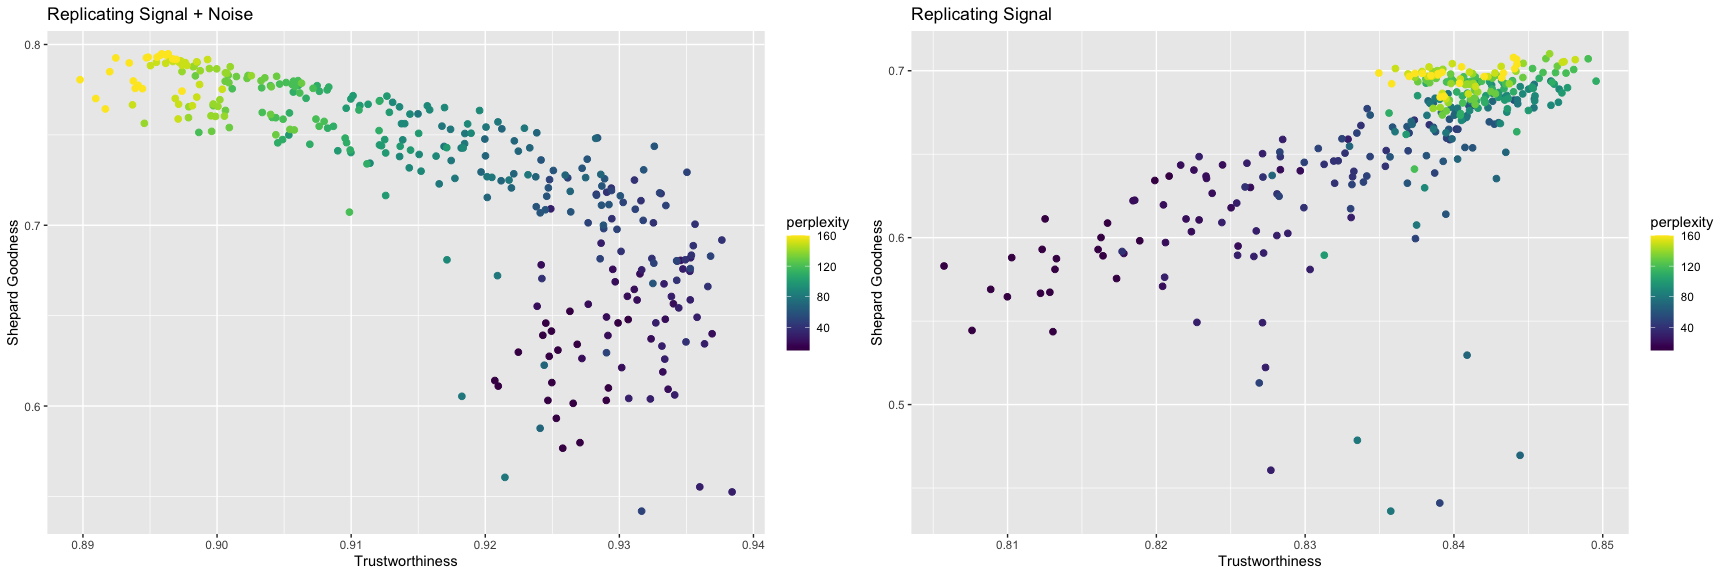
\includegraphics[scale=0.28]{links plot}
\caption{Shepard Goodness vs. Trustworthiness (Links)}
\end{figure*}

\renewcommand{\thefigure}{3b}
\begin{figure*}[t]
\centering
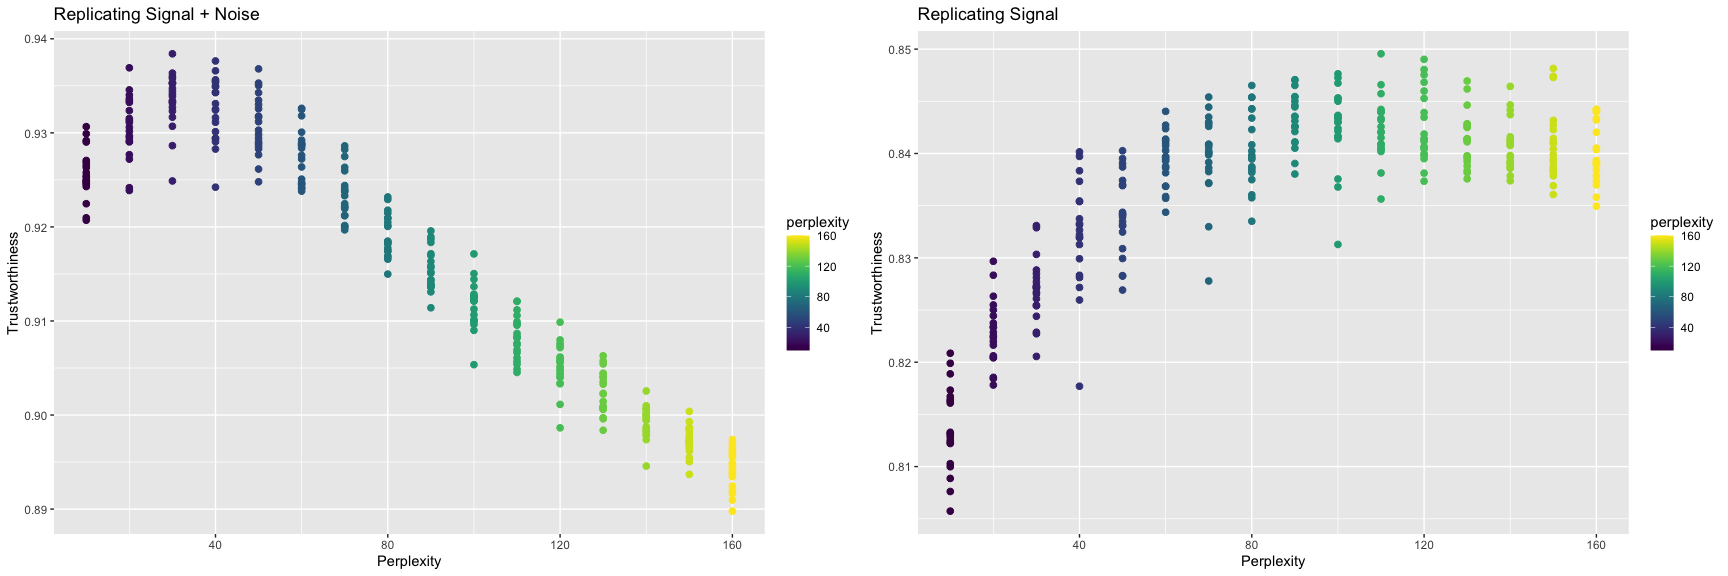
\includegraphics[scale=0.28]{trust plot (links)}
\caption{Trustworthiness vs. Perplexity (Links)}
\end{figure*}

Practical examples are more tricky because we do not have the luxury of first defining $Y$. Instead, we are given the data $Z + \epsilon$ from which we must extract $Y$, or at least our best estimate. This process is left to the researcher and should be based on a priori knowledge of the data. If there is no specific signal of interest, a more general approach can be taken. We used a PCA projection of the data to represent the signal, $$Y = \textrm{PCA}_r(Z + \epsilon),$$ where $r$ is the dimension of the projection. For a reasonable $r$, we would expect the first $r$ principal components to contain most of the signal, while excluding most of the noise. Another advantage to using PCA is it gives rise to a natural $\textrm{Emb}()$ function --- the PCA inverse transform. If $Y$ is centered, then we may define $$Z = \textrm{invPCA}_r(Y) = (Z + \epsilon)V_rV_r^T,$$ where $V_r \in \mathbb{R}^{p \times r}$ contains the first $r$ eigenvectors of $(Z+\epsilon)^T(Z+\epsilon)$ as column vectors.

\section{Results}

\subsection{Simulated Examples}
We first looked at simulated examples with explicitly defined signal structures: inter-linked circles, the trefoil knot, and the mammoth dataset (Figure 2).

\renewcommand{\thefigure}{2}
\begin{figure}[H]
\centering
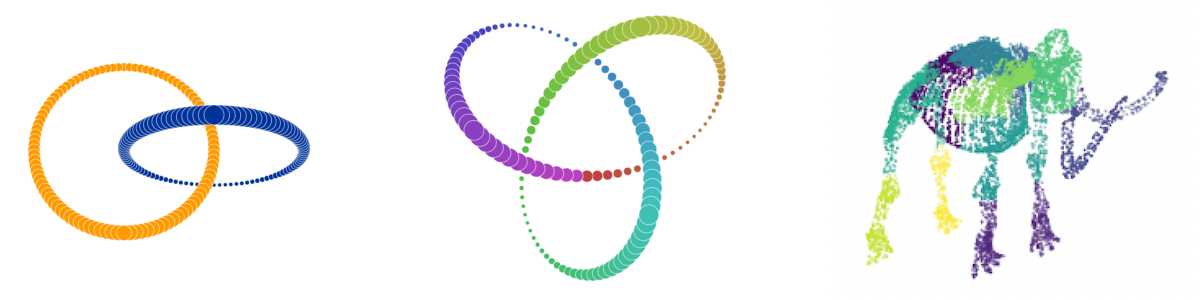
\includegraphics[scale=0.2]{simulated examples}
\caption{Simulated Examples; links and trefoil from (Wattenberg et al., 2016), mammoth from (Wang et al., 2021)}
\end{figure}

\renewcommand{\thefigure}{4a}
\begin{figure*}[b]
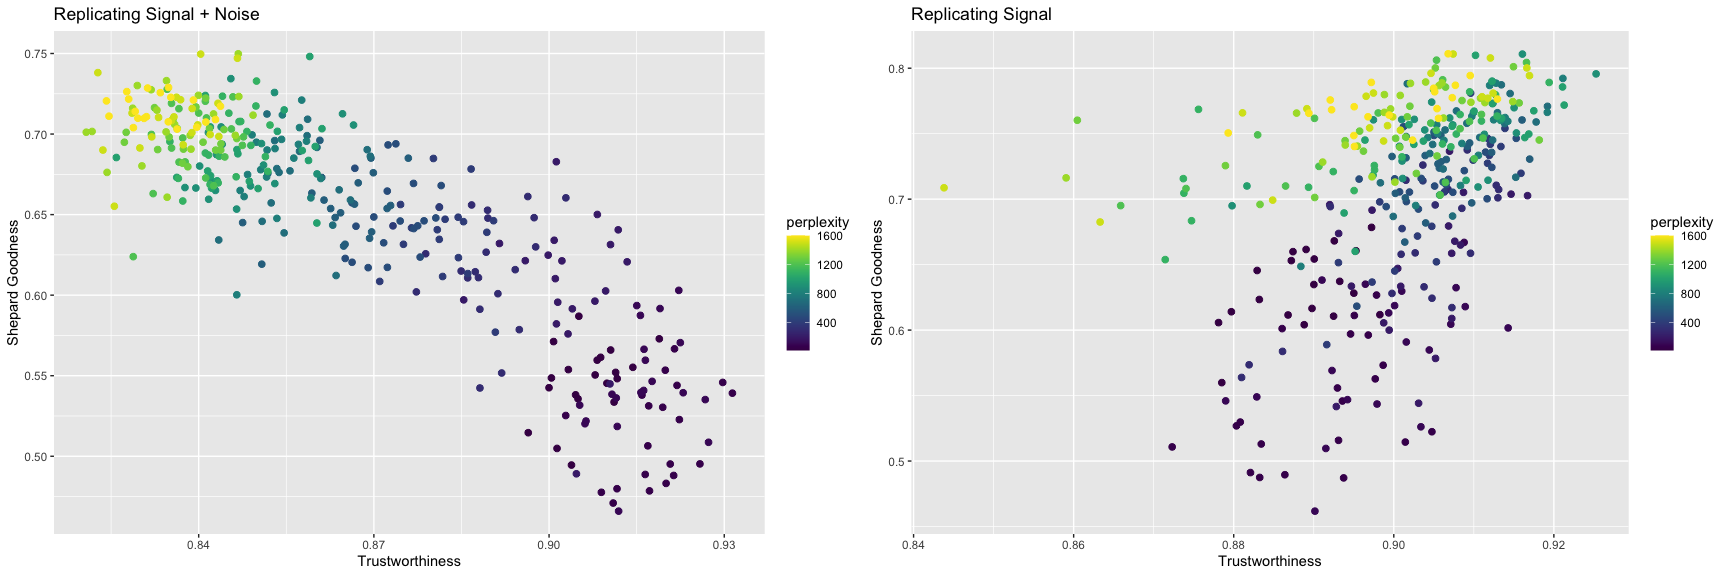
\includegraphics[scale=0.28]{CyTOF plot}
\centering
\caption{Shepard Goodness vs. Trustworthiness (CyTOF)}
\end{figure*}

\renewcommand{\thefigure}{4b}
\begin{figure*}[t]
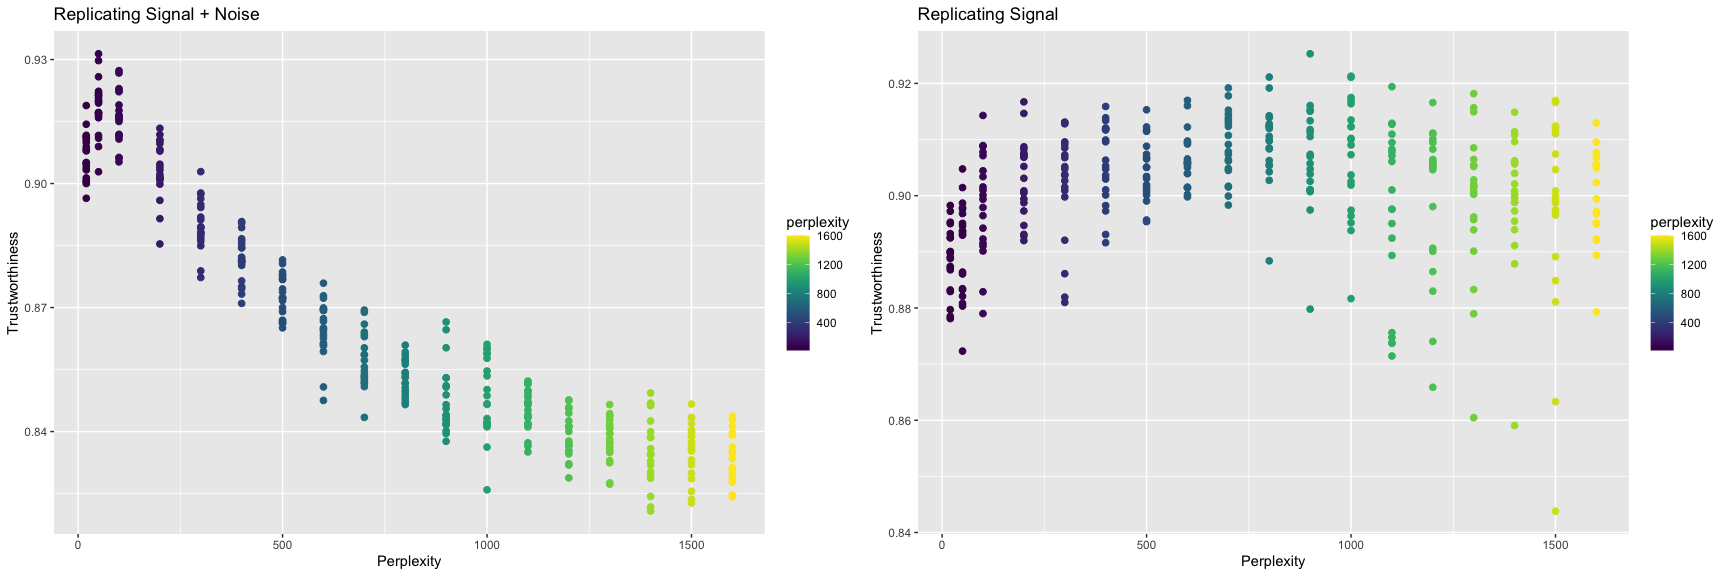
\includegraphics[scale=0.28]{trust plot (CyTOF)}
\centering
\caption{Trustworthiness vs. Perplexity (CyTOF)}
\end{figure*}

For each example, the signal $Y$ consisted of 500 points in three dimensions. The dataset $Z + \epsilon$ was constructed from $Y$ by adding seven superfluous dimensions and isotropic Gaussian noise to all 10 dimensions. We then ran t-SNE using the $R$ package \textit{Rtsne} with perplexities ranging from 10 to 160\footnote{\textit{Rtsne} implements a Barnes-Hut approximation that only allows for a maximum perplexity of $\frac{n-1}{3}$.}. For each value of perplexity, we ran the algorithm 20 times to mimic the ordinary t-SNE workflow. If we were to disregard the distinction between signal and noise, a plot of $f_\textrm{Shep}(Z + \epsilon, X)$ vs. $f_\textrm{trust}(Z + \epsilon, X)$ could be used to calibrate perplexity. To avoid overfitting the noise, a plot of $f_\textrm{Shep}(Y, X)$ vs. $f_\textrm{trust}(Y, X)$ should be used instead. See Figure 3a for plots of the links example. Both plots depict an increase in global performance as perplexity increases. Both plots also depict an increase in local performance followed by a decrease as perplexity increases. This trend is more evident when we plot trustworthiness vs. perplexity (Figure 3b).

Past a certain perplexity, local performance begins to deteriorate with increasing perplexity, exhibiting the trade-off between global and local performance. This cutoff point, however, varies between the two plots. When comparing against the original data, a perplexity of 30 maximizes trustworthiness, which is consistent with the original authors' suggestion of 5 to 50 for perplexity (van der Maaten and Hinton, 2008). When comparing against the signal, a perplexity of 110 maximizes trustworthiness. We hypothesize t-SNE tends to overfit the noise when the perplexity is too low. Intuitively, small perplexities are more affected by slight perturbations of the data when only considering small neighborhoods around each point, leading to unstable representations. Conversely, larger perplexities lead to more stable representations that are less affected by noise. The other two simulated examples exhibit a similar trend (See Supplementary Information).

\renewcommand{\thefigure}{5}
\begin{figure*}[b]
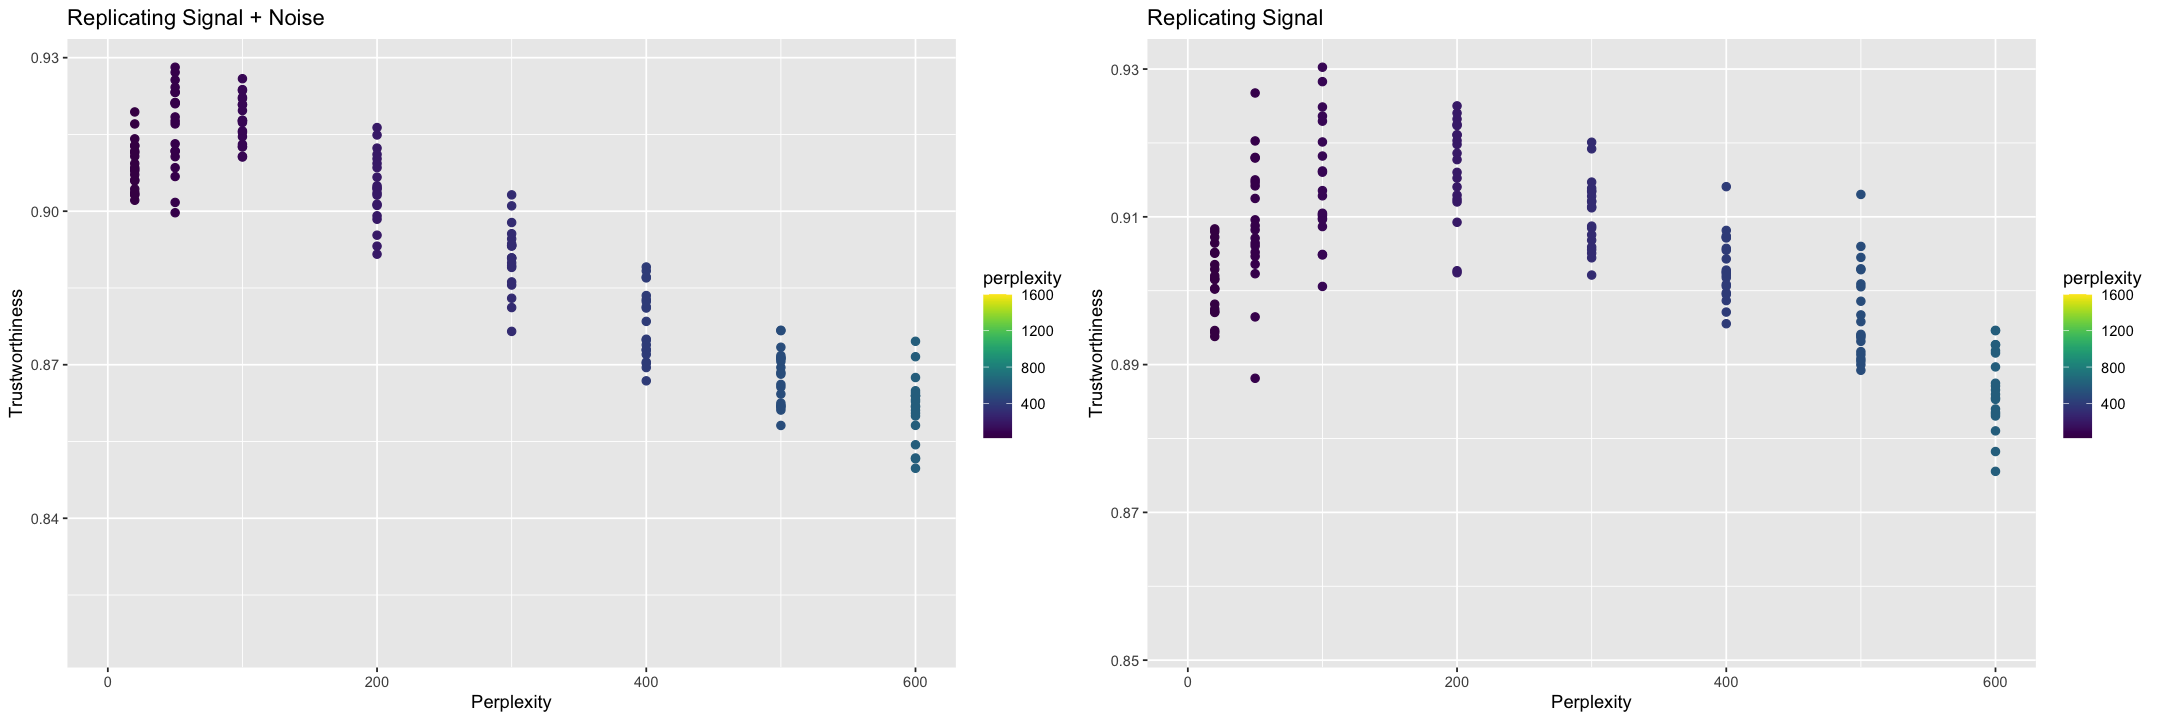
\includegraphics[scale=0.22]{5 dim plot (CyTOF)}
\centering
\caption{Trustworthiness vs. Perplexity for $r = 5$ (CyTOF)}
\end{figure*}

\subsection{Real Examples}
For a practical example, we looked at a CyTOF dataset containing 239,933 observations in 49 dimensions (Strauss-Albee et al., 2015). To reduce the computational load, a subset of 5,000 observations was sampled. In line with the ordinary t-SNE workflow, a log transformation was followed by a PCA pre-processing step to reduce the number of dimensions to 10. The processed data set to be studied consisted of 5,000 observations in 10 dimensions, $$Z + \epsilon \in \mathbb{R}^{5,000 \times 10}.$$  $Y$ was extracted by taking the first three principal components, $$Y = \textrm{PCA}_3(Z + \epsilon).$$ We computed the t-SNE representations for perplexity values ranging from 20 to 1,600. For each perplexity value, 20 different t-SNE representations were computed. Figure 4a contains the plots for $f_\textrm{Shep}(Z + \epsilon, X)$ vs. $f_\textrm{trust}(Z + \epsilon, X)$ and $f_\textrm{Shep}(Y, X)$ vs. $f_\textrm{trust}(Y, X)$.

As with the simulated examples, there is a difference in trend when the frame of reference is the original data versus when it's just the underlying signal. More specifically, the t-SNE representations better locally represent the original data for lower perplexities and better locally represent the underlying signal for larger perplexities (Figure 4b). When compared against the original data, trustworthiness is maximized at a perplexity of 50, which is consistent with (Kobak and Berens, 2019)'s recommendation of setting perplexity to $n/100$. When compared against the underlying signal, trustworthiness is maximized at a much larger perplexity of 900, reinforcing the hypothesis that lower values of perplexity may be overfitting the noise.

If we, instead, decide to be a little more conservative and use the first five principal components to represent the signal, we still see a similar trend (Figure 5). Trustworthiness still increases then decreases with perplexity. In this case, however, trustworthiness peaks at a perplexity of 100, less than before. By including two extra principal components in the signal, we're assuming the data contains less noise, allowing the model to be more aggressive during the fitting process. Further experimentation confirmed that the trustworthiness-maximizing perplexity decreased as we included more dimensions in the signal.

\subsection{UMAP and n\_neighbors}
If n\_neighbors functions similarly to perplexity, we'd expect small values of n\_neighbors to overfit the data as well. Our experiments suggest this to be the case, but to a lesser degree. An identical experiment was run using the Python package \textit{umap-learn}. n\_neighbor values ranging from 20 to 1,000 were tested on the same CyTOF data set. An n\_neighbors value of 20 maximized trustworthiness when comparing against the original data, but an n\_neighbors value of 600 maximized trustworthiness when comparing against the underlying signal (see Supplementary Information for plots). While the difference in local performance for different values of n\_neighbors was smaller, the UMAP results exhibited a similar trend. Local performance peaked at a larger value when compared against the underlying signal versus the original data.

\section{Application}
To apply this framework in practice, one must decide how to extract the signal from the data. The signal should include the features of the data one desires to retain throughout the dimension reduction process. When using a PCA projection to serve as the signal, one could draw a scree plot or employ a component selection algorithm such as parallel analysis to determine the dimension of the signal (Horn, 1965).

With a signal constructed, it remains to compute t-SNE outputs at varying perplexities. It's recommended that at least a couple outputs are computed for each perplexity to account for t-SNE's inherit randomness. For each output, one must calculate the trustworthiness and Shepard goodness with respect to the signal. From there, one can choose the representation with the desirable balance of local and global performance. See algorithm 1. Sample code is available at \url{https://github.com/JustinMLin/DR-Framework/}.

\begin{algorithm}[h]
\caption{Measuring Performance in the Presence of Noise}\label{algo1}
\begin{algorithmic}[1]
\Require original data $Z + \epsilon$, perplexities $\{p_1, \hdots, p_m\}$ to test, and neighborhood size $k$
\State $Y \Leftarrow \textrm{PCA}_r(Z + \epsilon)$
\State $\textrm{perplexities} \Leftarrow \{p_1, \hdots, p_m\}$
\For {perplexity in perplexities}
	\Loop
		\State $X\_tsne \Leftarrow \textrm{Rtsne}(Z + \epsilon, \textrm{perplexity})$
		\State $trust \Leftarrow \textrm{trustworthiness}(Y, X\_tsne, k)$
		\State $shep \Leftarrow \textrm{Shepard\_goodness}(Y, X\_tsne)$
	\EndLoop
\EndFor
\State Plot trustworthiness and Shepard goodness values
\State Choose output with desired balance of local and global performance
\end{algorithmic}
\end{algorithm}

It is worth noting that computational barriers may arise, especially for very large data sets. To alleviate such issues, trustworthiness and Shepard goodness can be approximated by subsampling before calculation. Furthermore, t-SNE is generally robust to small changes in perplexity (van der Maaten and Hinton, 2008), so checking a handful of different perplexities is sufficient. If computing the t-SNE representations is the limiting factor, the perplexity can be calibrated for a subsample of the data, instead. (Skrodzki et al., 2023) found that embedding a $\rho$-sample, where $\rho \in (0,1]$ is the sampling rate, with perplexity $\textrm{Perp}'$ gives a visual impression of embedding the original data with perplexity $$\textrm{\textrm{Perp}} = \frac{\textrm{Perp}'}{\rho}.$$ With these concessions, applying this framework to calibrate perplexity is feasible for data sets of any size.

\section{Discussion}
We have illustrated the importance of acknowledging noise when performing dimension reduction by studying the roles perplexity and n\_neighbors play in overfitting data. When using the original data to calibrate perplexity, our experiments agreed with perplexities previously recommended. When using just the signal, however, our experiments indicated that larger perplexities performed better. Low perplexities lead to overly-flexible t-SNE models that are heavily impacted by the presence of noise, while higher perplexities exhibit better performance due to increased stability. These considerations are especially important when working with heavily noised data, which are especially prevalent in the world of single-cell transcriptomics (Chu et al., 2022).

We have also presented a framework for modeling dimension reduction problems in the presence of noise. This framework can be used to study other hyperparameters and their relationships with noise. In the case when a specific signal structure is desired, this framework can be used to determine which dimension reduction method best preserves the desired structure. Further works should explore alternative methods for extracting the signal in way that preserves the desired structure.

\section{Data Availability}
All data and example code are freely available at \url{https://github.com/JustinMLin/DR-Framework/}.

\bibliographystyle{abbrvnat}
\bibliography{reference}

\begin{thebibliography}{10}

\bibitem{TriMap}
Ehsan Amid and Manfred K. Warmuth. 
\newblock TriMap: Large-scale dimensionality reduction using triplets. 
\newblock {\em arXiv preprint arXiv:1910.00204v2}, 2022.

\bibitem{perplexity vs kl}
Yanshuai Cao and Luyu Wang. 
\newblock Automatic selection of t-SNE perplexity.
\newblock {\em arXiv preprint arXiv:1708.03229.v1}, 2017.

\bibitem{large DR unreliable}
Tara Chari and Lior Pachter.
\newblock The specious art of single-cell genomics.
\newblock {\em PLoS Computational Biology 19(8):e1011288},  2023.

\bibitem{noise in single-cell data}
Shih-Kai Chu, Shilin Zhao, Yu Shyr, and Qi liu.
\newblock Comprehensive evaluation of noise reduction methods for single-cell RNA sequencing data.
\newblock {\em Briefings in Bioinformatics 23:2}, 2022.

\bibitem{perplexity-free t-SNE}
Francesco Crecchi, Cyril de Bodt, Michel Verleysen, John A. Lee, and Davide Bacciu.
\newblock Perplexity-free parametric t-SNE.
\newblock {\em arXiv preprint arXiv:2010.01359v1}, 2020.

\bibitem{quantitative survey}
Mateus Espadoto, Rafael M. Martins, Andreas Kerren, Nina S. T. Hirata, and Alexandru C. Telea.
\newblock Towards a quantitative survey of dimension reduction techniques.
\newblock {\em IEEE Transactions on Visualization and Computer Graphics 27:3}, 2021.

\bibitem{parallel analysis}
Horn, John L.
\newblock A rationale and test for the number of factors in factor analysis.
\newblock {\em Psychometrika 30:2 179-185}, 1965.

\bibitem{evaluation of DR transcriptomics}
Haiyang Huang, Yingfan Wang, Cynthia Rudin, and Edward P. Browne.
\newblock Towards a comprehensive evaluation of dimension reduction methods for transcriptomic data visualization.
\newblock {\em Communications Biology, 5:716}, 2022.

\bibitem{t-SNE cell}
Dmitry Kobak and Philipp Berens.
\newblock The art of using t-SNE for single-cell transcriptomics.
\newblock {\em Nature Communications, 10:5416}, 2019.

\bibitem{rank-based criteria}
John A. Lee and Michel Verleysen.
\newblock Quality assessment of dimensionality reduction: Rank-based criteria.
\newblock {\em Neurocomputing 72:1431 -- 1443}, 2009.

\bibitem{umap}
\newblock Leland McInnes, John Healy, and James Melville.
\newblock {\em arXiv preprint arXiv:1802.03426v3}, 2020.

\bibitem{precision score}
Tobias Schreck, Tatiana von Landesberger, and Sebastian Bremm.
\newblock Techniques for precision-based visual analysis of projected data.
\newblock {\em Sage 9:3}, 2012.

\bibitem{subsample t-SNE}
Martin Skrodzki, Nicolas Chaves-de-Plaza, Klaus Hildebrandt, Thomas H\"ollt, and Elmar Eisemann.
\newblock Tuning the perplexity for and computing sampling-based t-SNE embeddings.
\newblock {\em arXiv preprint arXiv:2308.15513v1}, 2023.

\bibitem{CyTOF data}
Dara M. Strauss-Albee, Julia Fukuyama, Emily C. Liang, Yi Yao, Justin A. Jarrell, Alison L. Drake, John Kinuthia, Ruth R. Montgomery, Grace John-Stewart, Susan Holmes, and Catherine A. Blish.
\newblock Human NK cell repertoire diversity reflects immune experience and correlates with viral susceptibility.
\newblock {\em Science Translational Medicine 7:297}, 2015.
 
\bibitem{t-SNE}
Laurens van der Maaten and Geoffrey Hinton.
\newblock Visualizing data using t-SNE.
\newblock {\em Journal of Machine Learning Research 9:2579 -- 2605}, 2008.

\bibitem{trustworthiness}
Jarkko Venna and Samuel Kaski.
\newblock Visualizing gene interaction graphs with local multidimensional scaling.
\newblock {\em European Symposium on Artificial Neural Networks}, 2006.

\bibitem{understanding DR}
Yingfan Wang, Haiyang Huang, Cynthia Rudin, and Yaron Shaposhnik.
\newblock Understanding how dimension reduction tools work: An empirical approach to deciphering t-SNE, UMAP, TriMap, and PaCMAP for data visualization.
\newblock {\em Journal of Machine Learning Research 22}, 2021.

\bibitem{Distill}
Martin Wattenberg, Fernanda Vi\'egas, and Ian Johnson.
\newblock How to Use t-SNE Effectively.
\newblock {\em Distill}, 2016.

\end{thebibliography}

\end{document}
